%% BioMed_Central_Tex_Template_v1.06
%%                                      %
%  bmc_article.tex            ver: 1.06 %
%                                       %

%%IMPORTANT: do not delete the first line of this template
%%It must be present to enable the BMC Submission system to
%%recognise this template!!

%%%%%%%%%%%%%%%%%%%%%%%%%%%%%%%%%%%%%%%%%
%%                                     %%
%%  LaTeX template for BioMed Central  %%
%%     journal article submissions     %%
%%                                     %%
%%          <8 June 2012>              %%
%%                                     %%
%%                                     %%
%%%%%%%%%%%%%%%%%%%%%%%%%%%%%%%%%%%%%%%%%


%%%%%%%%%%%%%%%%%%%%%%%%%%%%%%%%%%%%%%%%%%%%%%%%%%%%%%%%%%%%%%%%%%%%%
%%                                                                 %%
%% For instructions on how to fill out this Tex template           %%
%% document please refer to Readme.html and the instructions for   %%
%% authors page on the biomed central website                      %%
%% http://www.biomedcentral.com/info/authors/                      %%
%%                                                                 %%
%% Please do not use \input{...} to include other tex files.       %%
%% Submit your LaTeX manuscript as one .tex document.              %%
%%                                                                 %%
%% All additional figures and files should be attached             %%
%% separately and not embedded in the \TeX\ document itself.       %%
%%                                                                 %%
%% BioMed Central currently use the MikTex distribution of         %%
%% TeX for Windows) of TeX and LaTeX.  This is available from      %%
%% http://www.miktex.org                                           %%
%%                                                                 %%
%%%%%%%%%%%%%%%%%%%%%%%%%%%%%%%%%%%%%%%%%%%%%%%%%%%%%%%%%%%%%%%%%%%%%

%%% additional documentclass options:
%  [doublespacing]
%  [linenumbers]   - put the line numbers on margins

%%% loading packages, author definitions

\documentclass[twocolumn]{bmcart}% uncomment this for twocolumn layout and comment line below
%\documentclass{bmcart}

%%% Load packages
%\usepackage{amsthm,amsmath}
%\RequirePackage{natbib}
%\RequirePackage[authoryear]{natbib}% uncomment this for author-year bibliography
%\RequirePackage{hyperref}
\usepackage[utf8]{inputenc} %unicode support
%\usepackage[applemac]{inputenc} %applemac support if unicode package fails
%\usepackage[latin1]{inputenc} %UNIX support if unicode package fails

\usepackage{slashbox,pict2e}

\usepackage[ruled]{algorithm2e}
\usepackage{algpseudocode}

\usepackage{graphicx}
\usepackage{epstopdf}
\usepackage{url}\renewcommand{\baselinestretch}{1}
\usepackage{epsfig}
\usepackage{amsmath,amssymb}
\usepackage{multirow}
\usepackage{caption}
\usepackage{fancyvrb}
\usepackage{mathptmx}
\usepackage{alltt}
\usepackage{amsmath}
\usepackage{comment}
\usepackage{amsfonts}
%%%%%%%%%%%%%%%%%%%%%%%%%%%%%%%%%%%%%%%%%%%%%%%%%
%%                                             %%
%%  If you wish to display your graphics for   %%
%%  your own use using includegraphic or       %%
%%  includegraphics, then comment out the      %%
%%  following two lines of code.               %%
%%  NB: These line *must* be included when     %%
%%  submitting to BMC.                         %%
%%  All figure files must be submitted as      %%
%%  separate graphics through the BMC          %%
%%  submission process, not included in the    %%
%%  submitted article.                         %%
%%                                             %%
%%%%%%%%%%%%%%%%%%%%%%%%%%%%%%%%%%%%%%%%%%%%%%%%%
\usepackage{booktabs}
%\usepackage{tikz}
\usepackage{tabularx}
\usepackage{float}
\usepackage{array}
\usepackage{subcaption}
\usepackage[english]{babel}
%\newcolumntype{L}{>{\centering\arraybackslash}m{3cm}}
%\usepackage{lineno,hyperref}
\usepackage{amsthm}
\usepackage{lipsum,amsmath,multicol}
\usepackage{enumitem}
\usepackage{slashbox,pict2e}
\usepackage{array}
\usepackage{bbm}
\usepackage[normalem]{ulem}

%\def\includegraphic{}
%\def\includegraphics{}



%%% Put your definitions there:
\startlocaldefs
\endlocaldefs


%%% Begin ...
\begin{document}

%%% Start of article front matter
\begin{frontmatter}

\begin{fmbox}
\dochead{Research}

%%%%%%%%%%%%%%%%%%%%%%%%%%%%%%%%%%%%%%%%%%%%%%
%%                                          %%
%% Enter the title of your article here     %%
%%                                          %%
%%%%%%%%%%%%%%%%%%%%%%%%%%%%%%%%%%%%%%%%%%%%%%

\title{An SVM-based Framework for Detecting DoS Attacks in Virtualized Clouds under Changing Environment}

%%%%%%%%%%%%%%%%%%%%%%%%%%%%%%%%%%%%%%%%%%%%%%
%%                                          %%
%% Enter the authors here                   %%
%%                                          %%
%% Specify information, if available,       %%
%% in the form:                             %%
%%   <key>={<id1>,<id2>}                    %%
%%   <key>=                                 %%
%% Comment or delete the keys which are     %%
%% not used. Repeat \author command as much %%
%% as required.                             %%
%%                                          %%
%%%%%%%%%%%%%%%%%%%%%%%%%%%%%%%%%%%%%%%%%%%%%%

\author[
   addressref={aff1},                   % id's of addresses, e.g. {aff1,aff2}
   %corref={aff1},                       % id of corresponding address, if any
   %noteref={n1},                       % id's of article notes, if any
   email={adel.abusitta@polymtl.ca}     % email address
]{\inits{AB}\fnm{Adel} \snm{Abusitta}}
\author[
   addressref={aff2},
   corref={aff2},
   email={martine.bellaiche@polymtl.ca}
]{\inits{MB}\fnm{Martine} \snm{Bellaiche}}
\author[
   addressref={aff3},
   email={michel.dagenais@polymtl.ca}
]{\inits{MD}\fnm{Michel} \snm{Dagenais}}


%%%%%%%%%%%%%%%%%%%%%%%%%%%%%%%%%%%%%%%%%%%%%%
%%                                          %%
%% Enter the authors' addresses here        %%
%%                                          %%
%% Repeat \address commands as much as      %%
%% required.                                %%
%%                                          %%
%%%%%%%%%%%%%%%%%%%%%%%%%%%%%%%%%%%%%%%%%%%%%%

\address[id=aff1]{%                           % unique id
  \orgname{Department of Computer and Software Engineering, Polytechnique Montreal}, % university, etc
  \street{2900 Boulevard Edouard-Montpetit},
  \city{Montreal},                    %
  \postcode{QC H3T 1J4},                                % post or zip code                         % city
  \cny{Canada}                                    % country
}
\address[id=aff2]{%                           % unique id
  \orgname{Department of Computer and Software Engineering, Polytechnique Montreal}, % university, etc
  \street{2900 Boulevard Edouard-Montpetit},
  \city{Montreal},                    %
  \postcode{QC H3T 1J4},                                % post or zip code                         % city
  \cny{Canada}                                    % country
}
\address[id=aff3]{%                           % unique id
  \orgname{Department of Computer and Software Engineering, Polytechnique Montreal}, % university, etc
  \street{2900 Boulevard Edouard-Montpetit},
  \city{Montreal},                    %
  \postcode{QC H3T 1J4},                                % post or zip code                         % city
  \cny{Canada}                                    % country
}

%%%%%%%%%%%%%%%%%%%%%%%%%%%%%%%%%%%%%%%%%%%%%%
%%                                          %%
%% Enter short notes here                   %%
%%                                          %%
%% Short notes will be after addresses      %%
%% on first page.                           %%
%%                                          %%
%%%%%%%%%%%%%%%%%%%%%%%%%%%%%%%%%%%%%%%%%%%%%%

%\begin{artnotes}
%\note{Sample of title note}     % note to the article
%\note[id=n1]{Equal contributor} % note, connected to author
%\end{artnotes}

%\end{fmbox}% comment this for two column layout

%%%%%%%%%%%%%%%%%%%%%%%%%%%%%%%%%%%%%%%%%%%%%%
%%                                          %%
%% The Abstract begins here                 %%
%%                                          %%
%% Please refer to the Instructions for     %%
%% authors on http://www.biomedcentral.com  %%
%% and include the section headings         %%
%% accordingly for your article type.       %%
%%                                          %%
%%%%%%%%%%%%%%%%%%%%%%%%%%%%%%%%%%%%%%%%%%%%%%

\begin{abstractbox}

\begin{abstract} % abstract
Cloud Computing enables providers to rent out space on their virtual and physical infrastructures. Denial of Service (DoS)
attacks threaten the ability of the cloud to respond to clients' requests, which results in considerable economic losses. The existing detection approaches are still not mature enough to satisfy a cloud-based detection system's requirements since they overlook the changing/dynamic environment, that characterises the cloud as a result of its inherent characteristics. Indeed, the patterns extracted and used by the existing detection models to identify attacks, are limited to the current VMs’ infrastructure but do not necessarily hold after performing new adjustments according to the pay-as-you-go business model. Therefore, the accuracy of detection will be negatively affected. Motivated by this fact, we present a new approach for detecting DoS attacks in a virtualized cloud under changing environment. The proposed model enables monitoring and quantifying the effect of resources adjustments on the collected data. This helps filter out the effect of adjustments from the collected data and thus enhance the detection accuracy in dynamic environments. Our solution correlates as well VMs’ application metrics with the actual resources’ load, which enables the hypervisor to distinguish between benignant high load and DoS attacks. It helps also the hypervisor identify the compromised VMs that try to needlessly consume more resources. Experimental results show that our model is able to enhance the detection accuracy under changing environments.
\end{abstract}

%%%%%%%%%%%%%%%%%%%%%%%%%%%%%%%%%%%%%%%%%%%%%%
%%                                          %%
%% The keywords begin here                  %%
%%                                          %%
%% Put each keyword in separate \kwd{}.     %%
%%                                          %%
%%%%%%%%%%%%%%%%%%%%%%%%%%%%%%%%%%%%%%%%%%%%%%
\begin{keyword}
\kwd{Cloud Computing}
\kwd{DoS Attacks Detection}
\kwd{Support Vector Machine}
\kwd{Changing Environment}
\kwd{Virtual Machines}
\end{keyword}

% MSC classifications codes, if any
%\begin{keyword}[class=AMS]
%\kwd[Primary ]{}
%\kwd{}
%\kwd[; secondary ]{}
%\end{keyword}

\end{abstractbox}
%
\end{fmbox}% uncomment this for twcolumn layout

\end{frontmatter}

%%%%%%%%%%%%%%%%%%%%%%%%%%%%%%%%%%%%%%%%%%%%%%
%%                                          %%
%% The Main Body begins here                %%
%%                                          %%
%% Please refer to the instructions for     %%
%% authors on:                              %%
%% http://www.biomedcentral.com/info/authors%%
%% and include the section headings         %%
%% accordingly for your article type.       %%
%%                                          %%
%% See the Results and Discussion section   %%
%% for details on how to create sub-sections%%
%%                                          %%
%% use \cite{...} to cite references        %%
%%  \cite{koon} and                         %%
%%  \cite{oreg,khar,zvai,xjon,schn,pond}    %%
%%  \nocite{smith,marg,hunn,advi,koha,mouse}%%
%%                                          %%
%%%%%%%%%%%%%%%%%%%%%%%%%%%%%%%%%%%%%%%%%%%%%%

%%%%%%%%%%%%%%%%%%%%%%%%% start of article main body
% <put your article body there>

%%%%%%%%%%%%%%%%
%% Background %%
%%
\section*{Introduction}
Several major Information and Communications Technology (ICT) companies are competing for creating advanced cloud computing services that are able to deal with small, medium-sized and large-scale enterprise demands. Many companies, organizations and governments are expected to transfer, if not already done, all or parts of their IT solutions to the cloud \cite{Wong:2016} \cite{gonzales2015cloud}. This transfer is profitable from an economic point of view since it allows them to streamline the spending on technology infrastructure and capital cost. However, the security threat in terms of Denial of Service (DoS) attacks constitutes a major obstacle against the achievement of this transfer. A DoS attack can be of many types and may be seen in different contexts (e.g., application, web services, network) \cite{modi2013survey}. However, in this paper, we consider Virtual Machine (VM)-based DoS attacks in a virtualized cloud and define a DoS attack as follows. A DoS attack occurs when one or more VMs drain all the available physical resources such that the hypervisor would not be able to support more VMs \cite{tsai2012threat}. This attack is mainly caused by virtualization \cite{shea2012understanding} \cite{tsai2012threat}, which is the backbone of the recent cloud computing architecture, where virtualization allows emulating a particular computer system and sharing physical resources (e.g., CPU and network bandwidth).
In this paper, we shed light on the problem of detecting cloud-based DoS attacks under a changing environment. Although several advanced approaches have been proposed to detect DoS attacks in virtualized cloud (e.g., \cite{gupta2013vm} \cite{masood2013edos} \cite{koduru2013detection} \cite{kwon2011self}), these approaches still causes a significant decrease in the detection accuracy when used in a cloud environment. The reason is that the current approaches don't consider the changing environment, that characterises the cloud as a result of its inherent characteristics (resources restriction and scaling). Such characteristics are essential for the VM to meet the requirements of the pay-as-you-go business model \cite{wahab2017optimal}.

\subsection*{Motivating Example}
Assume that a cloud provider trained an Support Vector Machine (SVM) classifier on some VMs’ features under a certain infrastructure. These features include CPU, network, memory and I/O load. Assume now that the cloud provider, due to some business factors, decides to adjust some of the VMs' resources. This adjustment includes revoking 45\% from some VMs' resources. Such an adjustment will result in a significant decrease in the DoS detection accuracy rate. The reason is that the features used to train the SVM classifier were extracted under the original infrastructure (before revoking 45\% from VMs' resources). However, these features become unsuitable in the light of the new adjustment in the VMs resources. In other words, the collected data will be affected by the new adjustment, which will lead to an inaccurate classification of the collected data.

Indeed, the continuous requests to make adjustments on the infrastructure are necessary as long as the cloud client (e.g., VM) wants to meet the Quality of Service (QoS) requirements. The reason is that the ability of performing new adjustments, to cope with the real-time economic factors, affects the decision of the industries, organizations and governments on whether to adopt or not cloud computing. In other words, the continuous adjustments are necessary for the continuous use of the cloud to meet the variations in the demands and the cost-efficiency, which are considered as the main cloud features.

\subsection*{Our Proposed Solution}
To address the aforementioned problems, we propose a flexible detection framework based on the SVM learning technique. SVM is a classification technique that employs a nonlinear mapping to convert the original data into higher-dimensional of data, in order to find a hyperplane that optimally separates the training tuples based on their classes \cite{han2011data}. Our framework can be summarized as follows. The hypervisor collects some features to train the SVM classifier to be able to distinguish between the normal activity and DoS attack on the VM. The hypervisor then monitors and quantifies the effect of performing resources adjustments (i.e., granting/revoking resources to/from the VMs) on the collected VM's performance data. This information (i.e, effect of performing resources adjustments) is used thereafter to maintain a filter of resources adjustments effect. The filter is used as a preprocessing step, prior to classification, to get rid of the ``noise'' that may show up on the collected data (due to the new adjustments) and that may considerably decrease the accuracy of the detection.

Moreover, the proposed framework enables VMs to regularly declare their current application metrics, such as number of clients, requests and sales. This is then used by the hypervisor to correlate these metrics with the actual resources' load. This correlation enables the hypervisor to distinguish between benignant high load and DoS attacks. In addition, it enables the hypervisor to identify the compromised-VMs that may try to claim and consume more resources. We propose a correlation technique that the hypervisor uses to calculate the expected resources' load of the current compromised-VM's based on the declared metrics. The calculated resources' load is then compared with the actual resources' load. If the calculated resources' load is not within a certain range of the actual resources' load, the belief that the VM has been compromised increases. In summary, we propose a comprehensive framework that consists of the following contributions:

\begin{itemize}

\item Proposing a detection approach to identify DoS attacks in a virtualized cloud under changing environment. To the best of our knowledge, our work is unique in considering the detection problem under changing environment in virtualized clouds.

\item Proposing the monitoring and quantification of the effect of performing resources adjustments, which enhances the accuracy of identifying DoS attacks under changing environments.

\item Proposing a model to correlate VMs' metrics with the actual resources' load by the host, which enables the hypervisor to identify compromised VMs.

\item Modeling an incentive technique that enables the hypervisor to give incentives in the form of resources to the VMs that have truthfully declared their metrics and punish these VMs that lied about their actual metrics.

\end{itemize}

\subsection*{Paper Outline}
The rest of the paper is organized as follows. In section 2, we discuss the related work. In Section 3, we present the proposed framework. Section 4 presents security analysis of the proposed framework. In section 5, we present our empirical results. Finally, section 6 concludes the paper.


\section*{Related Work}

%\cite{lonea2013detecting}
Machine learning for detecting DoS attacks in the cloud was used by several researchers. This work benefits from many advanced machine learning and and artificial intelligence techniques to predict the status of VMs (i.e, malicious or normal).  For example, Lonea et al. \cite{lonea2013detecting} uses the normal traffic pattern received from the Virtual Bridge (VB) of the VM to validate for consistency against behavioral patterns of attacks. They use a network intrusion detection system, that analyzes the normal traffic flow obtained from the VB, to check and test for consistency against the attack behavioral patterns. Thus, if abnormal traffic has been detected, the anomaly information will be reported and an alarm generated.

%\cite{gupta2013vm} \cite{gupta2013vm} \cite{masood2013edos} \cite{koduru2013detection} \cite{kwon2011self}

Similarly, Gupta et al. \cite{gupta2013vm} propose a profile based network intrusion detection system. They combine both finen-grained data analysis and Bayesian techniques in order to detect TCP SYN flooding. The main advantage of these approaches is the ability to identify DoS symptoms at an early stage, because their approaches are able to collect information at the networking level, before the DoS causes a significant performance degradation. However, the lack of application performance information can result in wrongly identifying high traffic during the peak time as a DoS attack.

%\cite{masood2013edos}\cite{kwon2011self}
Masood et al. \cite{masood2013edos} propose a web-behavior-based detection, where they identify two client's profiles. The first one is for good clients while the second one is for bad clients. A good client will follow a pattern that reflects normal activity on the web, while a bad client will show some abnormal activities. Similarly, Anusha et al. \cite{koduru2013detection} study the behavior of normal users of Web applications. They assume that an attacker spends a very short time (almost zero) over a Web page. They use for that a metric called Time Spent on a Page (TSP). They assume that the attackers TSP is very close to zero. In contrast, the TSP of a normal client should be high enough to interact with the Web page. The work of Kwon et al. \cite{kwon2011self} also uses a behavioral approach for detection. They start from a tested assumption saying that the behavioral patterns of normal traffic are similar, while the behavior patterns of malicious traffic are not. The cosine similarity is used to check the similarity of the traffic. If such a similarity does not exist, an alarm is generated. A main advantage of this approach that it is able to determine the similarity during run-time. However, there is no guarantee that the normal traffic will always be similar in a dynamic environment (i.e. cloud). In fact, in some applications, we could have many forms of normal traffic that are fairly dissimilar.

%\cite{palmieri2014distributed}\cite{choi2014method}
Palmieri et al. \cite{palmieri2014distributed} use a two-phase ML-based detection technique. The first phase is called Blind Source Separation (BSS), while the second phase is called Rule-based Classifier to detect zero-day attacks that change or alter the traffic volume rate. BSS extracts the features of the cloud nodes traffic in order to be used by a decision tree classifier to create a normal traffic profile (baseline). Most recently, Choi et al. \cite{choi2014method} propose a data-mining-based approach to detect application layer HTTP GET DoS attacks. They use a normal behavior pattern to detect DoS attacks on VMs. The parameters used for analyzing and creating attack patterns are: CPU usage, packet size and packet header information. They evaluate their approach by comparing it with a signature-based approach. The result showed that their proposed method performs better than SNORT in terms of identifying new attack profiles. Similar to this work, Jeyanthi and Mogankumar \cite{jeyanthi2014virtual} and Jeyanthi et al. \cite{jeyanthi2013escape} propose a mechanism to detect DDoS attacks based on clients request rate. Clients requests will be put in a black list or white list based on a certain threshold rate. The threshold is determined by calculating the maximum number of legitimate client requests. The authors have shown experimentally that the legitimate clients could continue being served during an attack using their method. However, the main disadvantage of this method is that it is threshold based, where setting the optimal threshold is always difficult and infeasible in a production cloud environment.
%\cite{jeyanthi2013escape}\cite{jeyanthi2014virtual}

%\cite{chonka2012detecting}\cite{chonka2011cloud}

Chonka and Abawajy \cite{chonka2012detecting} and Chonka et al. \cite{chonka2011cloud} propose a decision tree classification technique. The method operates in two phases: training phase (first phase) and testing phase (second phase). In the training phase, a rule set that has been generated over time by the decision tree classifier is used to define both known and unknown attributes. In the testing phase, a decision making module is used to decide the likelihood of a previously classified packet. This helps decide whether to let a packet enter or not. Similar to that, Lonea et al. \cite{lonea2013detecting} also proposed a classification technique based on Intrusion detection system (IDS). The detection module analyse the alerts generated by each VM using the Dempster-Shaferther theory (quantitative solution classifier) in 3-valued logic and fault tree analysis (FTA). Although Dempster-Shaferther is able to produce powerful results when observations about attacks come from different sources, it becomes unsuitable when one source produces multiple observations \cite{wahab2014dempster}.

Among other approaches, the work of Iyengare et al. \cite{iyengar2014multilevel} proposes a Multilevel Thrust Filtration (MTF) that contains four detection and prevention modules, which are traffic analysis, anomaly detection, anomaly classification, and attack prevention. The proposed method filters the incoming packets and detects four types of traffic congestion, which are spoofing, ash crowd, DDoS, and aggressive legitimate traffic. A similar approach has been proposed by Jeyanthi and Iyengar \cite{jeyanthi2013escape}. The main feature of this approach is the ability to increase the attack detection accuracy because multiple stages of detection are used. However, it is associated with a significant overhead since multiple algorithms and techniques should be used.

The aforementioned work paved the way to understand the issues behind improving the detection accuracy in cloud environments. Our proposed model offers two major features. The first is the aspect of detection under changing environment. To the best of our knowledge, our work is the first to consider the detection problem under changing environment in virtualized clouds. The second is allowing VMs to share information about their current application metrics (e.g, number of clients, requests and sales) to the hypervisor, which in turn allows distinguishing between legitimate high load and DoS attacks. It also enables the hypervisor to identify the compromised-VMs that try to claim and consume more resources.


\section*{The Proposed Framework}
In this section, we describe the key constituents of our framework. The framework contains a set of components, each of which exhibits a set of modules. Figure 1 illustrates the framework structure and describes the modules of each component. These components include: data gathering, data and load analysis, and detection.

\begin{figure*}[!ht]
    \center
	\vspace{2mm}
	\scalebox{0.75}{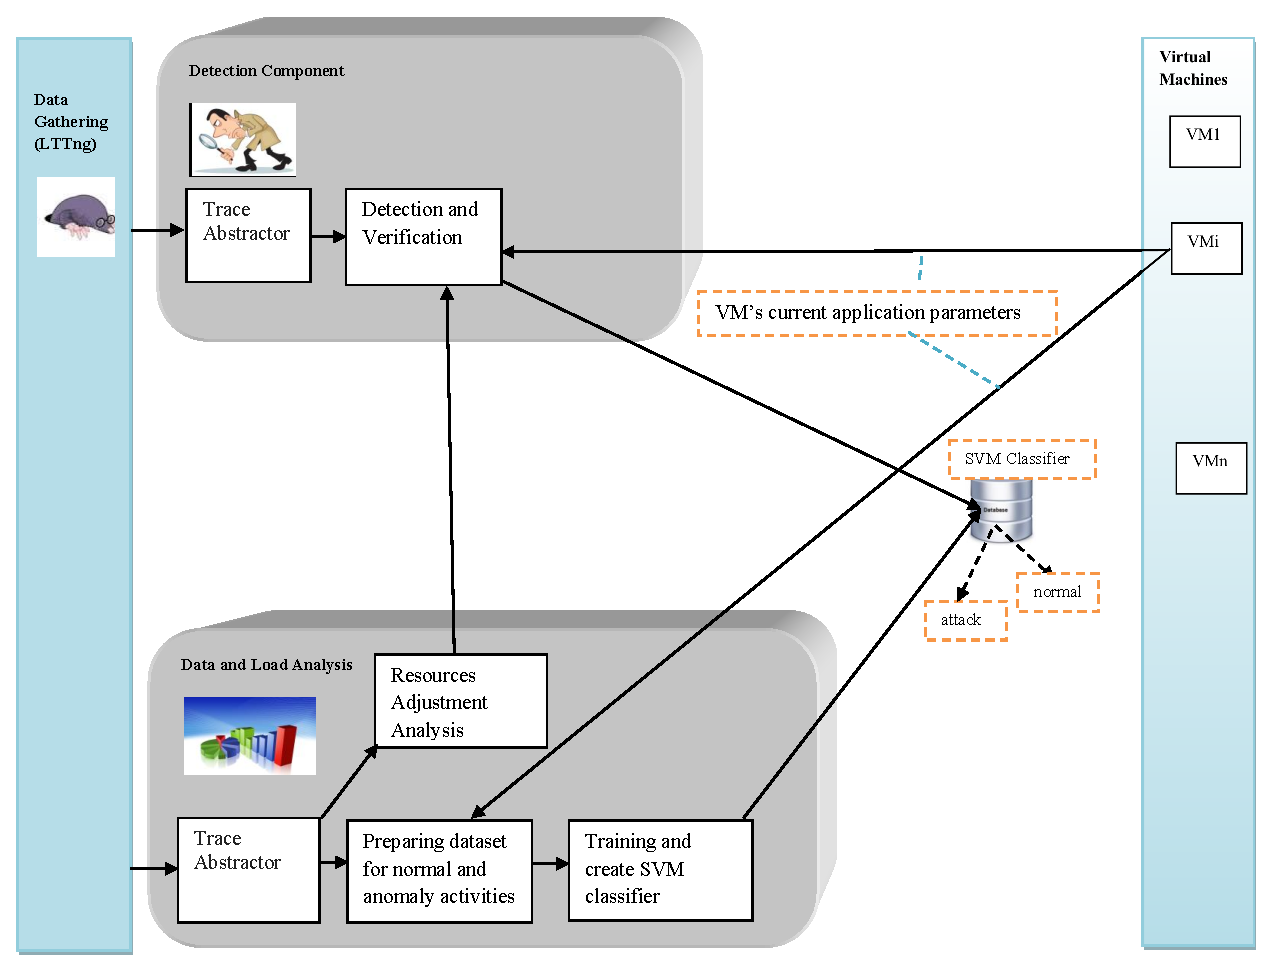
\includegraphics{model.eps}}
    \label{fig1}
    \caption{Architecture of the Proposed Framework}
\end{figure*}

We use the Linux Trace Toolkit next generation (LTTng) \cite{desnoyers2006lttng} to gather the VMs' performance metrics. LTTng is a powerful, low impact and lightweight \cite{ezzati2012stateful} open source Linux tracing tool. It provides precise and detailed information on the underlying kernel and user-space executions. LTTng contains different trace points in various modules of the operating system's kernel. Once a predefined trace point is reached, it generates an event containing a time-stamp, CPU number and other run-time information related to the running processes.

%\cite{desnoyers2006lttng}

\subsection*{Data Analysis}
This component is responsible for analysing data obtained from the data gathering component. We divide this component into the four modules: Trace abstractor, preparing dataset for normal and anomaly activities, training and create SVM classifier, and resources adjustment analysis.

\subsubsection*{Trace Abstractor}
The trace file size is usually so large that it is difficult to analyze and understand the system execution. Most of the time, another analysis tool is required to abstract the low-level events and represent them as higher-level events, thus reducing the data to be analyzed. Trace abstraction is typically required to compute statistics of complex system metrics that are not directly computable from the low-level trace events \cite{ezzati2013framework}. For instance, to compute synthetic  metrics such as ”number of HTTP connections”, ”CPU usage”, and ”number of different types of system and network attacks”, raw events must be aggregated to generate high-level events. Then, the desired metrics must be extracted and computed. Table 1 gives examples of a higher-level event generated from low-level events. The details of the trace abstraction tool used to generate such high-level meaningful events can be found in \cite{ezzati2012stateful}.

\begin{table}[ht]\small
\caption{Abstracting Example.}
\centering
 \begin{tabular}{c c}
 \hline
 \textbf{Low-level events} & \textbf{higher-level event} \\
\hline
  socket create  & HTTP connection\\
  socket call  & \\
  socket send & \\
  socket receive & \\
  socket close & \\
\end{tabular}
\end{table}

\subsubsection*{Preprocessing and Training Modules}

In this phase, the SVM \cite{han2011data} classification technique is used to analyse the collected data and classify the VMs' load. SVM is a classification technique that employs a nonlinear mapping to convert the original data into higher-dimensional data in order to find a hyperplane that best separates the training tuples based on their classes. The hyperplane is determined using support vectors and margins in such a way that maximizes the hyperplane's margins with the aim of delivering more accurate results when classifying future data tuples \cite{han2011data}. We use SVM thanks to its ability to generate very accurate classifiers (especially in  binary classifications) \cite{heller2003one} and its effectiveness in high dimensional datasets consisting of a large number of attributes \cite{shon2007hybrid}. Moreover, it is robust against outliers and overfitting \cite{wahab2015misbehavior} \cite{wahab2016ceap}.

The training dataset is generated during the monitoring of the host to determine which metrics reflect the malicious behavior and which ones reflect the normal behavior. As shown in the proposed architecture (Figure 1), VMs are allowed to share their application/business metrics to be considered among the features used to train the SVM. The VM's application/business metrics are discussed later in section 3.3.1.

Each VM can be either under DoS attack or normal. Thus, class label $y_{i}$ $\in$ $\{$attack, normal$\}$. Given the training datasets  ($x_{i}$,$y_{i}$)...($x_{n}$,$y_{n}$), $x_{i}$ is the VM's metrics values used for the training. $n$ is the number of metrics values, the objective is to find the hyperline that offers a maximum margin (Figure 2) such that:

\begin{equation}\small
  w \ast x + b = 0
\end{equation}



Where $w$ is a weight vector (Eq. 6) and $b$ is a threshold.

Thus, the training data should satisfy:

\begin{equation}\small
  w \ast x_{i} + b \geq -1 \hspace{0.3cm} for \hspace{0.3cm} all \hspace{0.3cm} attack \hspace{0.3cm}data \hspace{0.3cm} x_{i}
\end{equation}

\begin{equation}\small
  w \ast x_{i} + b \leq +1 \hspace{0.3cm} for \hspace{0.3cm} all \hspace{0.3cm} normal \hspace{0.3cm}data \hspace{0.3cm} x_{i}
\end{equation}


The problem is converted to finding the optimal hyperplane (Eq. 1), which can be turned into a convex optimization problem \cite{scholkopf2002learning}:


\begin{figure}[!ht]

    \center
	\vspace{2mm}
	\scalebox{0.25}{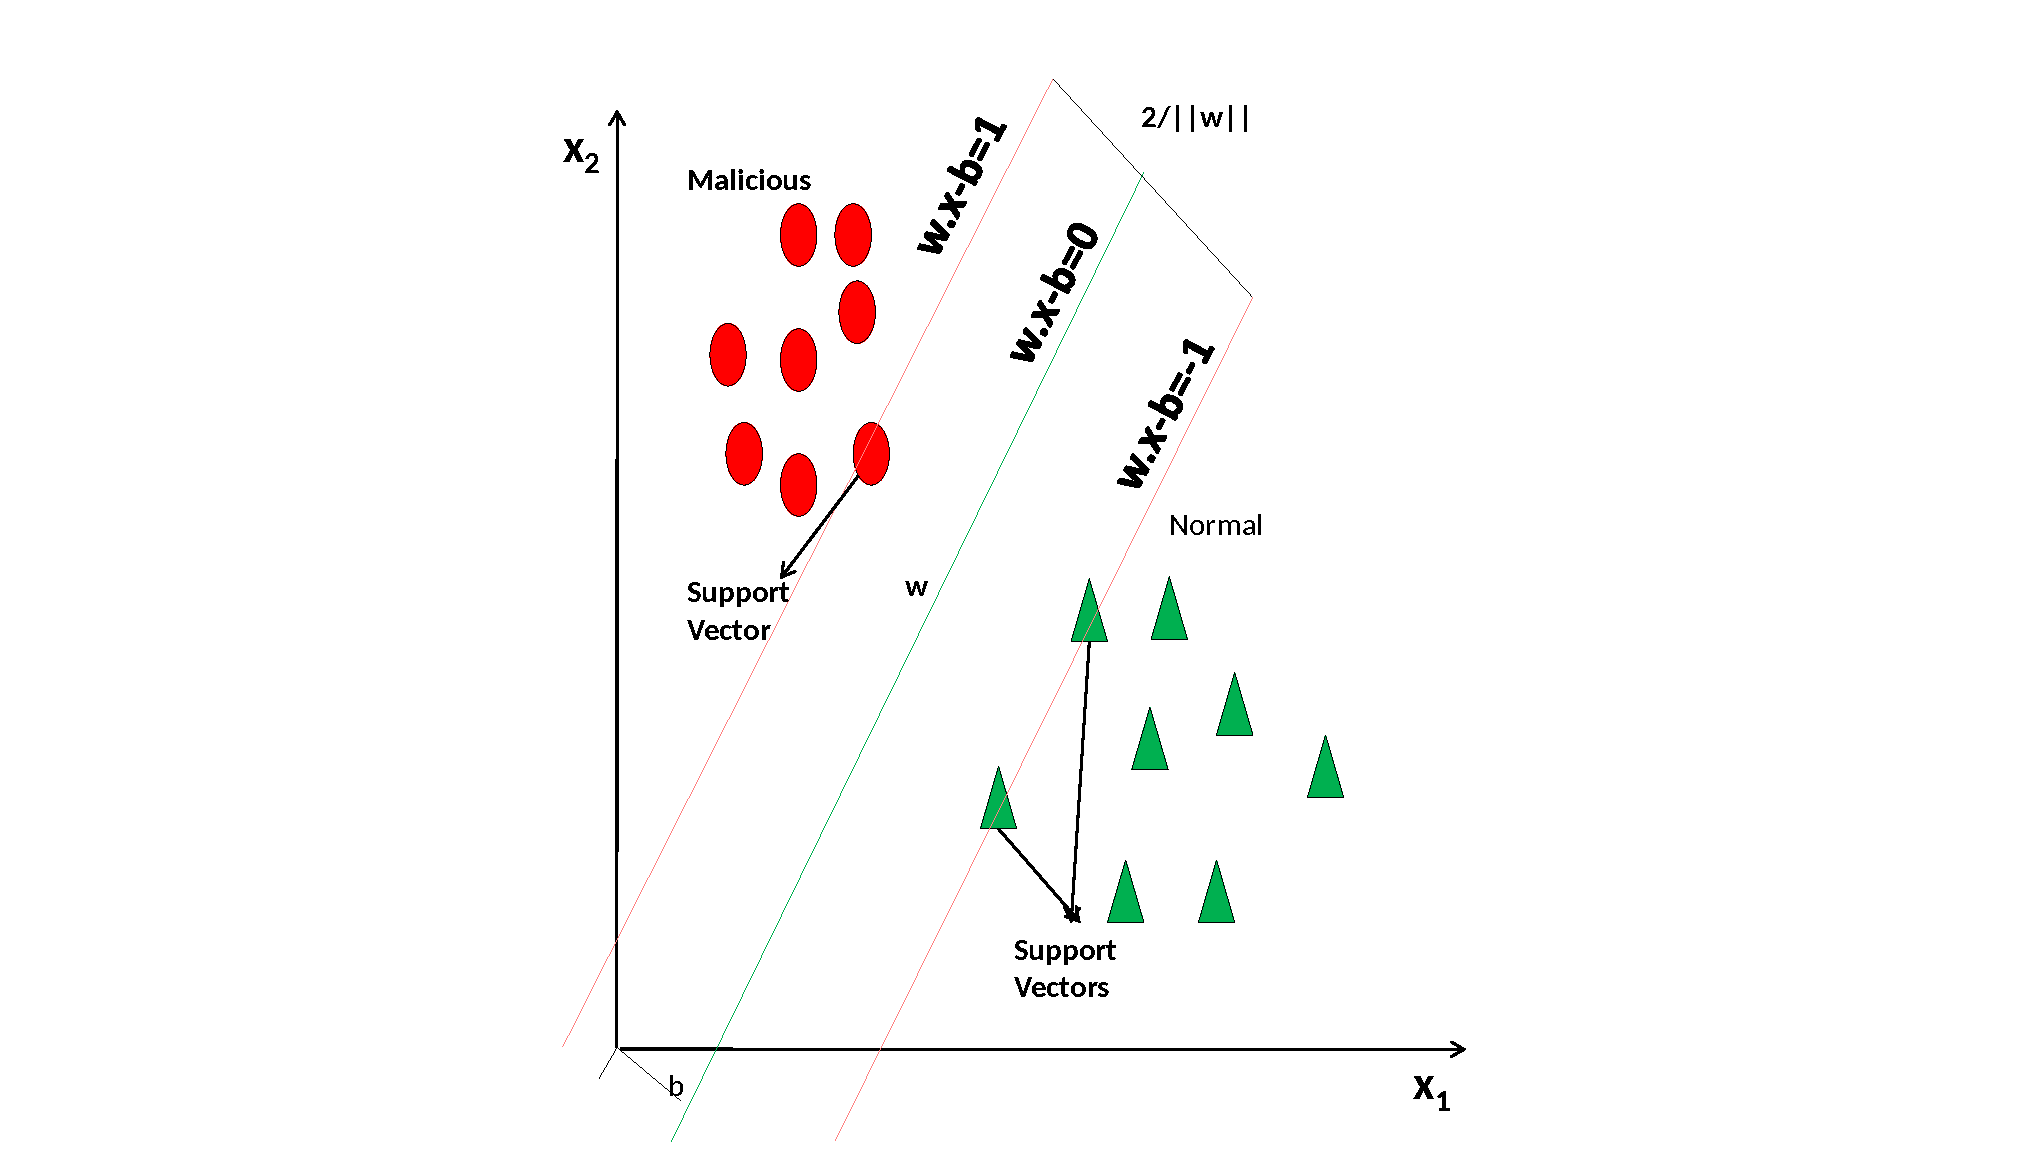
\includegraphics{SVM.eps}}
    \label{fig1}
    \caption{The value of w affects the position of the hyperplane.}
\end{figure}
\vspace{2mm}

%\cite{shon2007hybrid}\cite{wahab2015misbehavior

\begin{equation}\small
  \left\{
  \begin{aligned}
  &min \hspace{0.3cm} \tau(w)={\frac{\|w\|}{2}} \\
  &Subject \hspace{0.3cm} to \hspace{0.3cm}  y_{i}(\langle w, x_{i}\rangle + b) \hspace{0.3cm} for \hspace{0.3cm} all \hspace{0.3cm} i= 1,...,n
  \end{aligned}
  \right\}
\end{equation}

The convex optimization can be solved using Lagrange multipliers  \cite{scholkopf2002learning}:
\begin{equation}\small
  \left\{
  \begin{aligned}
  &maximize \hspace{0.3cm} L(\alpha) = \sum_{i=1}^{n}\alpha_{i}-\frac{1}{2}\sum_{j=1}^{n} \sum_{i=1}^{n} \alpha_{i}\alpha_{j}y_{i}y_{j}K(x_{i},x_{j}) \\
  &Subject \hspace{0.3cm} to \hspace{0.3cm} \sum_{i=1}^{n}y_{i}\alpha_{i}=0 \hspace{0.3cm} and \hspace{0.3cm} 0 \leq \alpha_{i}\leq C \hspace{0.3cm} \forall \hspace{0.3cm} 1\leq i \leq n
  \end{aligned}
  \right\}
\end{equation}

where $\alpha_{i}$ is the Lagrange multipliers \cite{han2011data}, $K$($x_{i}$,$x_{j}$) represents the kernel function (e.g., linear, polynomial, etc.) and C is a constant for determining the trade-off between margin maximization and training error minimization \cite{han2011data}.

By solving Eq. 5 we get \cite{han2011data}:

\begin{equation}\small
  w = \sum_{i=1}^{n} \alpha_{i}y_{i}x_{i}
\end{equation}

Finally, the decision attack function is given by:

\begin{equation}
f(x,\alpha,b)= \{\pm1\}=sgn(\sum_{i=1}^{n} y_{i}\alpha_{i}K(x,x_{i}) + b)
\end{equation}

\subsubsection*{Resources Adjustment Analysis}

The impact of resources adjustment appears on the collected data, which makes the SVM classifier unsuitable in the light of the new adjustment in the VMs resources. In other words, the collected data will be affected by the new adjustments, which leads to an inaccurate classification of that data. To address this issue, we should determine the effect of resources adjustment on the collected data (we will discuss later in this section how to calculate the effect of resources adjustments). The effect of resources adjustment reflects to what extent the modified data (after new resources adjustment) deviates from the original data (the data that meets the basic infrastructure).

Having the effect of resources adjustment, two approaches to solve the detection problem under changing environment can be considered. The first approach is to consider this effect during the training of the SVM classifier. This can be done by generating new sub features for every feature (features represent system metrics in this context) used in the training. In fact, the new sub features are the result of applying the effect of resources adjustment on the basic feature. For example, if the original feature used to train the SVM classifier is 10, 20, 30, 40 for CPU, memory, I/O, and network respectively, then the SVM classifier is also trained to classify in the presence of 50\% adjustment on the VM's resources by adding to the training set the following new sub feature: (10 + 10 * 50\%), (20 + 20 * 50\%), (30 + 30 * 50\%) and (40 + 40 * 50\%) for CPU, memory, I/O, and network respectively. This makes the SVM classifier be trained not only on the original infrastructure but also on the new infrastructure after resources adjustment.

The second approach is to account for the resources adjustments effect by a separate filter. The filter is used as a preprocessing step, prior to classification, to get rid of the effect of resources adjustment on the collected data, in order to normalise the data with respect to the original infrastructure on which the training was performed, before passing it to the SVM classifier. We adopt the second approach in the proposed framework for the two following reasons. On the one hand, the first approach requires generating a huge training dataset, since we have to generate many sub-features for each single feature. This results in more overhead during the SVM training. The second approach does not require any change in the dataset. On the other hand, training an SVM with all possible adjustments (as is the case for the first approach) may lead to an overfitting. Specifically, the classifier might work correctly in the presence of the trained adjustment; However, the classifier accuracy will go down in the absence of such adjustments.

\paragraph{The Effect of Resources Adjustment.}

The effect of resources adjustment on VMs is studied during the running of the VMs to find out to what extent their system metrics are affected by the adjustments. Although such a process requires changing the VMs' resources which in turn may affect the performance of the application running inside these VMs, the impact of an adjusting and monitoring the effect is acceptable since it is done during a short time period ($\approx$ the time needed to capture VMs' system metrics). Note that resources adjustment process can be done by exploring and monitoring the effect of all possible resources adjustments performed on VMs' system metrics. More specifically, we maintain a filter of resources adjustments effect (as in Figure 3), which is used as a preprocessing step prior to classification (i.e., SVM), to filter out the effect of resources adjustments from the collected data. In other words, this helps to get rid of the noise that may show up on the collected data (due to the new adjustments) and may considerably decrease the accuracy of the detection. Algorithm 1 is used to determine the effect of all possible resources adjustments on the VM's system metrics.

%In addition, resources adjustment is not limited to revoking resources from the VM,


\begin{figure*}[!ht]
    \center
	\vspace{-10mm}
	\scalebox{0.65}{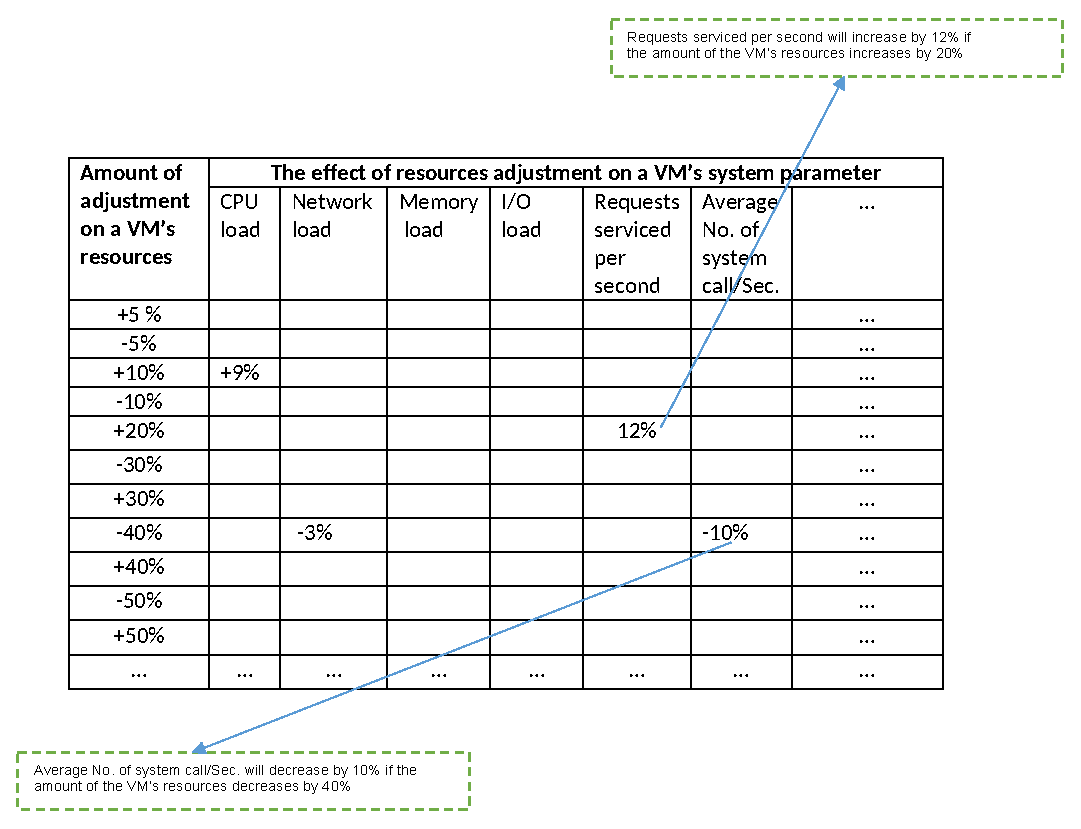
\includegraphics{adjustment.eps}}
    \label{fig1}
    \caption{Table used for filtering out the effect of resources adjustments on a VM's system metrics.}
\end{figure*}

\begin{algorithm}[h]
\LinesNumbered
\SetKwInOut{Input}{Input}\SetKwInOut{Output}{Output}
\Input{List of VMs' possible resources adjustment $adj$[]}
\Output{The effect of resources adjustment on VMs' system metrics $\{$$eff_{1}$[][],$eff_{2}$[][], ... , $eff_{n}$[][]$\}$}

%\While{$\varepsilon$ has not elapsed}
\Repeat{$\varepsilon$ elapses}
{
\ForEach{Running VM $j$}
{

      Monitor and store $j$' system metrics in array $U_{1}$ (before adjustments)

   \ForEach{Adjustment $adj$ $\in$ $adj$ []}
   {

      Apply an adjustment of amount $adj$ on $j$'s resources

      Monitor and store $j$' system metrics in array $U_{2}$

      Remove the adjustment of amount $adj$ and restore $j$'s default resources

   \ForEach{index $i$ of $U_{1}$}
   {
        $BeforeAdj$ = $U_{1}$[$i$] \\
        $AfterAdj$ = $U_{2}$[$i$] \\

        \uIf{$|BeforeAdj -  AfterAdj|$ $<$ $\epsilon$}
        {
          $eff_{j}$[$adj$][$i$] = 0
        }
        \uElseIf{$BeforeAdj$ $<$ $AfterAdj$}
        {
          $eff_{j}$[$adj$][$i$] = $\frac{adj*100}{AfterAdj}  * BeforeAdj$
        }
        \Else {
          $eff_{j}$[$adj$][$i$] = - $\frac{adj*100}{AfterAdj}  * BeforeAdj$
        }
   }
   }
}
}


\caption{Determining the effect resources adjustment on VMs' system metrics.}
\end{algorithm}

In Algorithm 1, for each $VM^{j}$ ($j$ $\in$ VMs) in a certain host, the algorithm monitors and determines the current system metrics of $j$ to be stored in array $U_{1}$ [] (line 3). Then, for each possible resources adjustment $adj$, the algorithm applies resources adjustment of value $adj$, to see the effect of $adj$ on $j$'s system metrics. Note that we apply adjustments on VMs' resources using control groups (cgroups) \cite{cgroups:2016}, which is a Linux Kernel feature that limits and allocates resources to VMs — such as CPU time, system memory, network bandwidth, or combinations of these resources. The system metrics are re-computed after each adjustment process (line 6). Then, the algorithm computes the effect of an adjustment $adj$ on VM $j$'s system metrics by finding the percentage of change on the $j$'s system metrics (line 8 - 16). If the new calculated metric $U_{2}$ [$i$]'s value is within a small range of the old value $U_{1}$[$i$], the effect will be considered as 0. This is described in the Algorithm 1 as $eff_{j}$[$adj$][$i$] = 0 (line 12), which means that the effect of an adjustment $adj$ on that $i$-th metric of VM $j$ is equal to 0. This indicates that the resources adjustment had no effect on that given metric. However, if the new calculated metric's value considerably differs from the old one, the algorithm computes the percentage of change on the old value such that: $eff_{j}$[$adj$][$i$] = $\frac{adj*100}{AfterAdj}  * BeforeAdj$ (line 14) for a positive change (i.e., new-value $>$ old-value) and - $\frac{adj*100}{AfterAdj}  * BeforeAdj$ (line 16) for a negative change (i.e., new-value  $<$ old-value). The algorithm is used for each possible adjustment in order to have a filter of resources adjustments effect for each VM. The filter is then used during the detection step (Section 3.3) to filter out the collected data from the effect of resources adjustment. This adapts the environment of the detection to the original environment (i.e., the environment in which the SVM classifier was created). Note that the whole process is repeated periodically after a certain fixed period of time $\varepsilon$ (line 17) to capture the new effect of the given resources adjustment on VMs' system metrics.

The main computation complexity of Algorithm 1 is during the calculation of the effect of resources adjustment on each VM's system metrics (line 8 - 16), which is $O(n)$, where $n$ is the number of VM's system metrics.

It should also be noticed that some resources adjustment may have no impact on VMs' system metrics. In fact, it can depend on resources and the underlying usage model. For example, for a given load,  if we consume 60\% of the CPU (100\% available with no restriction), when a restriction of 70\% is imposed, we will consume 60\% / 70\% = 85\% of the available CPU. The number of CPU seconds will remain the same though. For this purpose, we have considered in the resource adjustment algorithm the following condition: If ($|BeforeAdj -  AfterAdj|$ $<$ $\epsilon$) (line 11), which means that the collected data are the same before and after adjustments. The effect of resources adjustment in this case is equals to 0, as given in Algorithm 1 ($eff_{j}$[$adj$][$i$] = 0).


\subsection*{Detection Component}

This component is used for identifying DoS attacks. It monitors the system and performs tracing abstraction, similar to the steps used in section 3.1 and section 3.2.1. Along with these steps, the module performs the detection algorithm described in Algorithm 2. The following section presents the details of this component.

\subsubsection*{Detection Algorithm}

Algorithm 2 that is used for detecting DoS attacks works as follows. For each $VM^{j}$ ($j$ $\in$ VMs) in a certain host, the algorithm uses the model obtained from section 3.3.1 to calculate the VM's resources' load (calculated load) with respect to the VM's declared metrics (line 4). This step is important to minimise unnecessary false positive alarms during flash events. The calculated resources' load is compared with the actual resources' load to determine if the calculated resources' load is within a small range of the actual resources' load (line 5). If this is not the case, the detection process starts by filtering out the effect of resources adjustment on $j$'s system metrics using $j$'s resources adjustment effect (given as input in Algorithm 2) (i.e.,  $newU[i]$ = $U[i]$ $\pm$ ($U[i]$ * $eff_{j}$[$VMA^{j}$][$i$]) (line 6-10) from the collected data. The objective is to adjust the data for the original infrastructure on which the training was performed before passing it to the SVM classifier. The Algorithm passes then the modified collected data to SVM to predict the result (line 11). If the result $r$ = "attack", the algorithm identifies a DoS attack (line 12-13). If the calculated resources' load is within a short distance of the actual load, the algorithm identifies the resources' load as normal (line 16-17).

\begin{algorithm}[h]
\LinesNumbered

\SetKwInOut{Input}{Input}\SetKwInOut{Output}{Output}
\Input{VMs' alpha values $\{$$\alpha_{1}$, $\alpha_{2}$, ..., $\alpha_{n}$$\}$}
\Input{VMs' beta values $\{$$\beta_{1}$, $\beta_{2}$, ..., $\beta_{n}$$\}$}
\Input{VMs' declared application metrics $VMT^{j} \hspace{0.3cm} \forall \hspace{0.1cm} j \in VMs$}
\Input{VMs' effect of resources adjustment on their system metrics $\{$$eff_{1}$[][], $eff_{2}$[][], ..., $eff_{n}$[][]$\}$}
\Input{Amount of adjustment applied to VMs' resources $VMA^{j} \hspace{0.3cm}\forall\hspace{0.1cm} j \in VMs$}
\Output{Attack Boolean $Dec$}

\ForEach{VM $j$}
{
Determine $j$'s current resources' load $crt\_load$.


Monitor and store $j$'s system metrics in array $U$.


$calc\_load$= $\alpha_{j}$ + $\beta_{j}$ * $VMT^{j}$.

\If{$|calc\_load - crt\_load| > \epsilon$}{

     \ForEach{index $i$ of $U$}{

     \uIf{$eff_{j}$[$VMA^{j}$][$i$] $\geq$ 0}{
     $newU$[$i$] = $U$[$i$] - ($U$[$i$] * $eff_{j}$[$VMA^{j}$][$i$])

     }
     \Else{
      $newU$[$i$] = $U$[$i$] + ($U$[$i$] * $eff_{j}$[$VMA^{j}$][$i$])
      }
      }
      \tcc{classifying data (i.e., newU using the SVM}
     $r$ = $predict(newU,SVM)$

     \If{$r$=="attack"}{
    $Dec$ = True

     }

     \Else{
     $Dec$ = False
     }

   }
   }
\Else
{
$Dec$ = False
}


\caption{Detection Algorithm}
\end{algorithm}

The main complexity of Algorithm 2 lies in three parts. In the first part, the algorithm filters out the effect of resources adjustment from the collected data (line 6-10). The computation complexity for this part is $O(n)$, where $n$ is the number of SVM's input metrics. The second part is to find if the predicted and calculated VM's resources' load are similar (line 5), which is of constant time complexity $O(1)$. The last part of the algorithm is to predict the modified collected data using SVM (line 11), the computational complexity of SVM-based prediction is $O(n)$, where $n$ is also the number of SVM's input metrics. Therefore, the overall computation complexity of the proposed detection Algorithm is $O(n) + O(n) + O(1)$ $\approx$ $O(n)$.

We don't consider here the time complexity of the SVM training, which is commonly known to be $O(n^{3})$ \cite{wahab2016ceap}, where $n$ represents the training set size. Although this might be infeasible for very large datasets, the training process is performed only once, and its overhead can then be neglected \cite{auria2008support} \cite{konar2005supervised}. Moreover, recently, more and more techniques are being proposed for efficient SVM training \cite{fine2001efficient} \cite{tsang2005core} \cite{dong2005fast}.

\subsubsection*{Verification and Resources Allocation}

The proposed detection framework allows a VM to regularly declare its current application metrics, which enables the hypervisor to correlate these metrics with the actual resources' load and decide if it is coherent or not (compromised VM trying to claim and consume more resources). In fact, the VM may have no incentive to declare its metrics. Moreover, the VM may lie about its current metrics either because of its selfish strategy (in order to obtain more resources) or because the VM has been compromised.

\begin{algorithm}[h]
    \SetKwInput{Initialization}{Initialisation}
    \LinesNumbered
    \Initialization{}
\SetKwInOut{Input}{Input}\SetKwInOut{Output}{Output}
\Input {VMs' alpha values $\{$$\alpha_{1}$, $\alpha_{2}$, ..., $\alpha_{n}$$\}$}
\Input {VMs' beta values $\{$$\beta_{1}$, $\beta_{2}$, ..., $\beta_{n}$$\}$}
\Input{VMs' declared application metrics $VMT^{j} \hspace{0.3cm} \forall \hspace{0.1cm} j \in VMs$}
\Output{Amount of resources granted/revoked to/from each VM}

\ForEach{VM $j$}
{
Determine $j$'s current resources' load $crt\_load$

$calc\_load$= $\alpha_{j}$ + $\beta_{j}$ * $VMT^{j}$

\If{$|calc\_load - crt\_load| < \epsilon$}
{
        Grant resources to $j$
}

\Else
{
        Revoke resources from $j$

}
}
\caption{Verification and Resources Allocation Algorithm}
\end{algorithm}

To address the aforementioned problems, we propose a verification algorithm (Algorithm 3). Our solution motivates the VM to declare its current application metrics by granting resources to the VM whose calculated resources' load (obtained from the VM's declared metrics) falls within a close range of the VM's actual resources' load (line 4-5). On the other hand, the hypervisor revokes resources from the VM whose calculated resources' load and actual resources' load do not match (line 6-7). This dissimilarity, in most cases, is either because the VM has lied about its declared metrics, or because the VM has been compromised. The amount of resources revoked from the VM can be decided by the system administrator, who clearly knows the real impact of adjusting the VM's resources on their performance. However, we suggest that the amount be proportional to the magnitude of the difference between the calculated resources' load and the current resources' load. In other words, the larger the difference between the calculated resources' load and current resources' load is, the more resources should be revoked from the VM. This encourages VMs to truthfully declare their metrics used to calculate the resources' load.

As for the complexity of Algorithm 3, the main computation complexity of the verification algorithm is to verify if the calculated resources' load is within a short distance of the current resources' load and apply a resources allocation according to line 4 -7, which is a constant complexity $O(1)$.

\section*{Security Analysis of the Proposed Framework}

The main objective of the proposed framework is to enhance the detection of DoS attacks under changing environment. In this section, we analyse the effectiveness of our framework in the presence of flash events, DoS attacks and compromised VMs.

\subsection*{Flash Events}

A flash event occurs when there is an unusual surge of legitimate traffic. Our model is able to distinguish  between a flash event and DoS attacks since our framework allows VMs to declare their current application metrics (e.g., number of clients) and motivates them to do that by granting them extra resources (Algorithm 3). The declared metrics can represent flash events. The declared metrics are then used to calculate the resources' load according to the model in section 3.3.1. The calculated and actual resources' load are then compared to see if they approximately match. If so, the hypervisor will know and understand that the VM is under an unusual surge of legitimate requests and will grant the VM more resources to serve better during this period. Otherwise, if the calculated and actual resources' load are largely different, the hypervisor revokes some resources from the VM. This strategy motivates the VM to truthfully declare its peak load and limit the illegal use of resources by the attacker, in case the VM has been compromised.

\subsection*{DoS Attacks}

The main purpose of the proposed framework is to detect DoS attacks. Our model achieves this by using SVM. The framework trains SVM classifiers on the normal and malicious features to achieve the learning of the classifier. Our framework then monitors the incoming features and predicts the system's status. Moreover, the proposed detection algorithm supports the detection under a changing infrastructure. The algorithm checks if no modification in the VM's resources (i.e., granting or revoking resources) has occurred. If so, the algorithm passes the collected data directly to the SVM classifier, without applying any filtering strategy. Otherwise, the algorithm filters the effect of resources adjustments in order to adjust the collected data to the original infrastructure (on which the training was performed), before passing it to the SVM classifier. This is done by removing the effect of noise caused by resources adjustments.

\emph{Proposition:} The accuracy of the detection will not be affected after filtering out the effect of resources adjustment.

\begin{proof}

Consider that the collected data $U$ has been affected by resources adjustment in such a way that makes $U$ change by percentage $\%eff$. The $\%eff$ can be a positive (e.g., +5\%), negative (e.g., -5\%) or 0 (as the example given in section 3.2.3, where some adjustments (e.g., CPU) don't result in any change in the collected data) . If $\%eff $ is positive, the value of $U$ changes to $U +(\%eff*U)$. In this case, our detection algorithm removes the adjustment (Algorithm 2 line 5-9) as follows:

\begin{equation}
 U+(\%eff*U) - (\%eff*U) = U
\end{equation}

On the other hand, if $\%eff$ is negative, the value of $U$ changes to $U$ - (\%eff*$U$). In this case, the detection algorithm removes the adjustment (As in Algorithm 2) as follows:

\begin{equation}
 U-(\%eff*U) +(\%eff*U) = U
\end{equation}

Also, if $\%eff$ = 0, the value of $U$ changes to $U$ - (0 * $U$) = $U$. In this case, the detection algorithm removes the adjustment as follows:

\begin{equation}
 U-(0 * U) +(0 * U) = U
\end{equation}

In the aforementioned three situations, the collected data $U$ can be recovered, which means that the detection will be performed as if no adjustment had been applied.
\end{proof}

\subsection*{Robustness against Compromised VMs}

The proposed framework is able to detect the compromised-VMs that try to claim receiving an unusual load of client requests, to be allowed to consume more resources. The compromised-VM can hide that its compromised by mimicking normal load and/or flash crowds \cite{kandula2005botz}. The hypervisor calculates the VM's load (resources' load) based on the compromised-VM's current declared application metrics and compares it with the actual resources' load. If the calculated resources' load is not within a short range of the actual resources' load, there will be a high probability that the VM has been compromised. A possible strategy that a compromised-VM may use, is trying to find $\alpha$ and $\beta$ in order to obtain the model for calculating the resources' load $load = \alpha + \beta * VM\_par$. This can be done by using different values of $\alpha$ and $\beta$. For every $\alpha$ and $\beta$, the compromised-VM sees the response from the hypervisor (the response is the resources given for the unusual declared metrics). If the compromised-VM did not receive a response, the compromised-VM tries other values of $\alpha$ and $\beta$, until the correct $\alpha$ and $\beta$ values are obtained (receiving a response from the hypervisor). Although this can be possible, the number of trials will be very high, which makes it infeasible for the attacker, since $\alpha$ and $\beta$ can be any real number from a large interval. In addition, the attacker will typically not have the opportunity to do a large number of attempts in trying to guess $\alpha$ and $\beta$. After several wrong guesses (e.g., 10 wrong attempts), the hypervisor would consider the VM as a compromised and prevent it from using resources.

\section*{Experimental Results and Analysis}

In this section, we first explain the experimental setup used to perform our experimentation and then study the performance of the proposed detection approach.

\subsection*{Experimental Setup}


To evaluate our model, we chose to create our custom test environment. Our testbed consists of three machines. One machine is used as a virtual machine host and the other machines are used as client and attack emulator. All machines are attached directly to a Linksys 1000 Mb/s SOHO switch. Our test network is completely disconnected from the network of our institution as well as from the Internet to avoid the leakage of the DoS attacks. The detection algorithm (Algorithm 2) is implemented in Python and the BoNeSi program is used \cite{Markus:2015} to generate attack-level and normal traffic. We used BoNeSi as a traffic generation tool because it allows us to simulate floods from large-scale bot networks. Moreover, BoNeSi tries to avoid the generation of packets with easily identifiable patterns, which can be quickly filtered out \cite{Markus:2015}. The virtual machine host used in the experiment is an Intel Core i7-4790 CPU 3.60 GHz Processor with 16 GB RAM. We installed the Apache 2.2 Web Server on the targeted VMs. The network interface is at 1000 Mb/s. We chose KVM \cite{KVM:2016} as our hypervisor-based virtualization. Indeed, KVM runs on the unmodified Linux kernel and is thus compatible with the standard performance tracing tools (e.g., LTTng), unlike Xen.

In order to simulate a real-world DoS attack, the CAIDA “DDoS Attack 2007” dataset \cite{Hick:2007} has been used as a baseline for extracting the features required to simulate attack traffic.  Since it is not possible to mine normal traffic data from CAIDA's dataset because it
is collected at Darknet and has no normal traffic, we used another dataset to capture normal traffic. For this purpose, we used a traffic trace of a 5-minute non-flash-event activity before the first semi-final match of the 1998 FIFA World Cup’ dataset \cite{Arlitt:1998}. Table 2 shows the traffic features and characteristics extracted from the CAIDA and  1998 FIFA World Cup’ datasets (the same features used in \cite{bhatia2014framework}). We used then BoNeSi as a traffic generator to be run based on information given in Table 2.

\begin{table}[ht]\small
\caption{Attack and normal traffic features extracted from CAIDA and FIFA World Cup’ datasets }
\centering
 \begin{tabular}{c c c}
 \hline
 \textbf{Characteristic} & \textbf{DoS Attacks}  & \textbf{Normal Traffic}  \\
\hline
 \textbf{Packet Size} &  64k & 64k\\
 \textbf{No. of Sources} & 859 & 73 \\
 \textbf{packet rate}  &  125,705 & 385 \\
\end{tabular}
\end{table}

\subsection*{Training Phase}

During the generation of the attack and normal traffic using BoNeSi, we monitored the following metrics: CPU, memory, I/O and network load at different time intervals. We can also monitor and use high-level metrics, as illustrated in the trace abstractor section (section 3.2.1). However, we prefer to use these relatively basic metrics as they are widely used to describe the anomaly caused by a DoS attack \cite{modi2013survey}. The length of each interval is 30 seconds. For each interval, we used LTTng to generate the trace data. To extract CPU, memory, I/O and network loads from the trace data, we used the LTTng-analyses packages \cite{lttng:2016}, which are a set of executable analyses to extract and visualise monitoring data and metrics from LTTng kernel traces. We created a training dataset that contains these performance metrics. The dataset is used then to train the SVM classifier to be able to distinguish between normal behavior and DoS attacks of the VM. We train an SVM classifier on our dataset using the 10-fold cross-validation model. We used a linear kernel function as it is considered more efficient for real-time applications \cite{maji2013efficient}. It enjoys as well faster training and classification. Moreover, with the linear function, less memory is required as compared to the non-linear kernels \cite{maji2013efficient}.


\subsection*{Testing Phase}

In order to test the proposed model in the presence of resources adjustments, we created a testing dataset that is suitable for each type of adjustments. To do this, we monitored the metrics (CPU, memory, I/O and network load) in the same way used to generate the training dataset. However, in this phase, we performed some resources adjustments on the VMs during data collection, in order to study the effectiveness of our proposed model in such a case. We used the API of libvirt that employs cgroups \cite{libvirt:2016} to adjust and limit VMs' resources. Using cgroups allows exploiting Linux Kernel features that limit and allocate resources to VMs — such as CPU time, system memory, network bandwidth, or combinations of these resources \cite{cgroups:2016}. This is performed on the two types of traffic datasets: attack and normal traffic. Our detection algorithm (Algorithm 2) is then executed on these datasets. The detection algorithm applies the filter of resources adjustment effect (obtained from executing Algorithm 1) on the testing dataset before passing it to the SVM classifier. The length of time used to determine the effect of resources adjustment in Algorithm 1 is 30 seconds.

We used to evaluate the accuracy of the proposed model the false positive, false negative, attack detection and accuracy rate.


Accuracy Rate =

\begin{equation}\small
100\% \times \frac{ Total\hspace{0.1cm}\#\hspace{0.1cm}of\hspace{0.1cm}correctly\hspace{0.1cm}classified\hspace{0.1cm}tuples}{Total\hspace{0.1cm}\#\hspace{0.1cm}of\hspace{0.1cm} tuples}
\end{equation}

Attack Detection Rate =

\begin{equation}\small
100\% \times \frac{ Total\hspace{0.1cm}\#\hspace{0.1cm}of\hspace{0.1cm}attacks}{Total\hspace{0.1cm}\#\hspace{0.1cm}of\hspace{0.1cm}detected\hspace{0.1cm}attacks}
\end{equation}

False Positive Rate =
\begin{equation}\small
 100\% \times \frac{ Total\hspace{0.1cm}\#\hspace{0.1cm}of\hspace{0.1cm}misclassified\hspace{0.1cm}tuples}{Total\hspace{0.1cm}\#\hspace{0.1cm}of\hspace{0.1cm}normal\hspace{0.1cm} tuples}
\end{equation}

False Negative Rate =

\begin{equation}\small
100\% \times \frac{ Total\hspace{0.1cm}\#\hspace{0.1cm}of\hspace{0.1cm}misclassified\hspace{0.1cm}tuples}{Total\hspace{0.1cm}\#\hspace{0.1cm}of\hspace{0.1cm}attack\hspace{0.1cm}tuples}
\end{equation}

The next section contains the results, compared to the traditional SVM \cite{han2011data} and Decision-Tree detection \cite{dobra2009decision} techniques. The traditional-SVM uses the SVM classifier directly, without applying any filtering strategy that can cope with the effect of the resources adjustment on the detection performance. Similarly, the Decision-Tree detection technique employs the Decision-Tree classification technique, without applying any filtering process. We train the traditional-SVM and Decision-Tree classifier on our dataset using the 10 fold cross-validation model.

\subsection*{Experimental Results}

\begin{figure}[!ht]
	\scalebox{0.40}{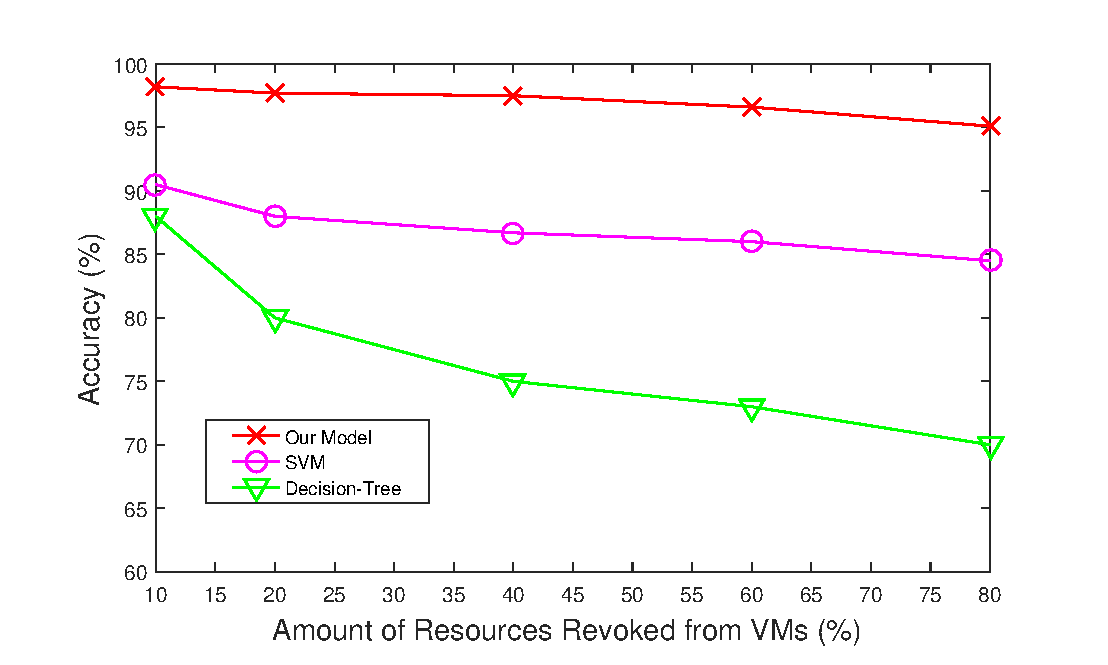
\includegraphics{revaccuracy.eps}}
    \label{fig1}
    \caption{Accuracy with respect to (w.r.t.) amount of revoked resources}
\end{figure}

\begin{figure}[!ht]
	\scalebox{0.40}{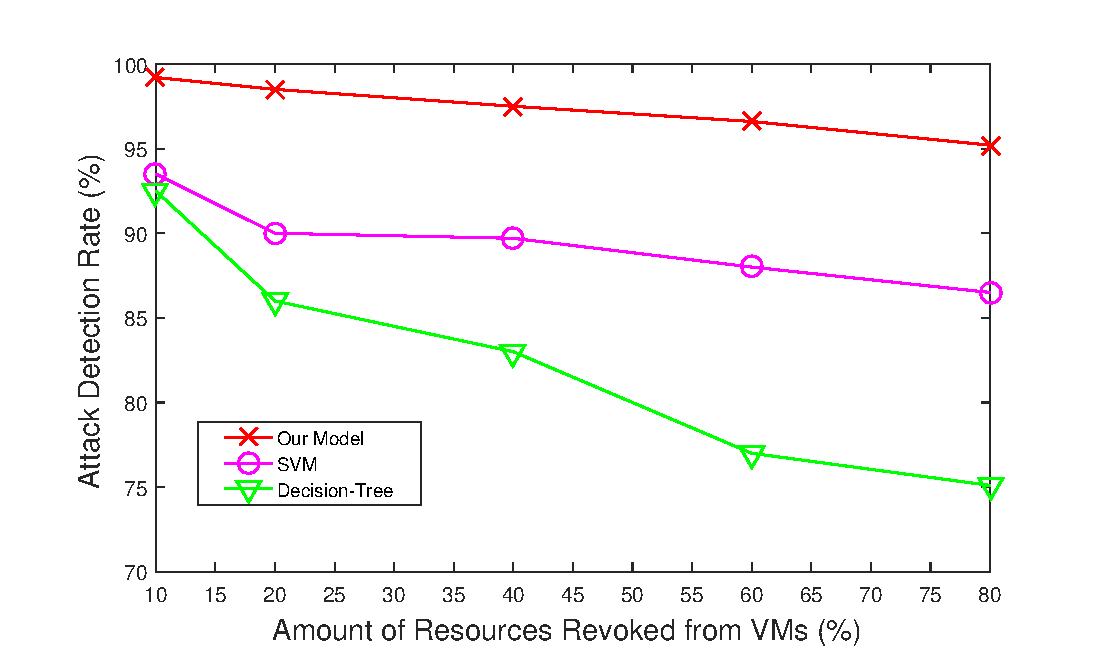
\includegraphics{revattackdetection.eps}}
    \label{fig1}
    \caption{Attack detection rate w.r.t. amount of revoked resources}
\end{figure}

\begin{figure}[!ht]
	\scalebox{0.40}{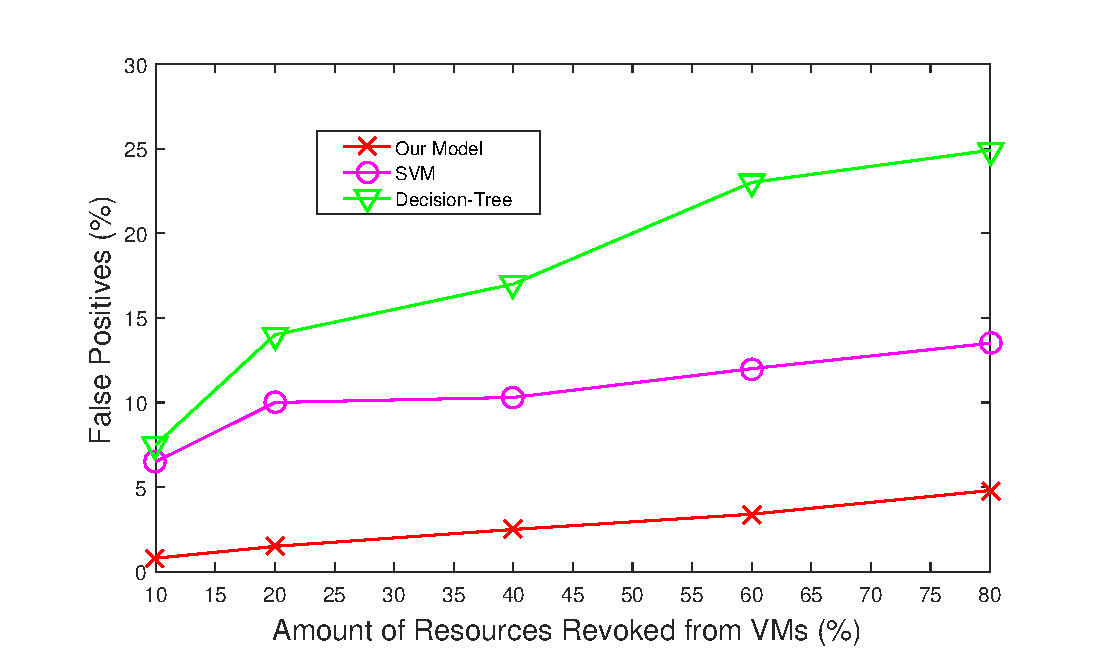
\includegraphics{revfalsepositive.eps}}
    \label{fig1}
    \caption{False positive percentage w.r.t. amount of revoked resources}
\end{figure}
\begin{figure}[!ht]
	\scalebox{0.40}{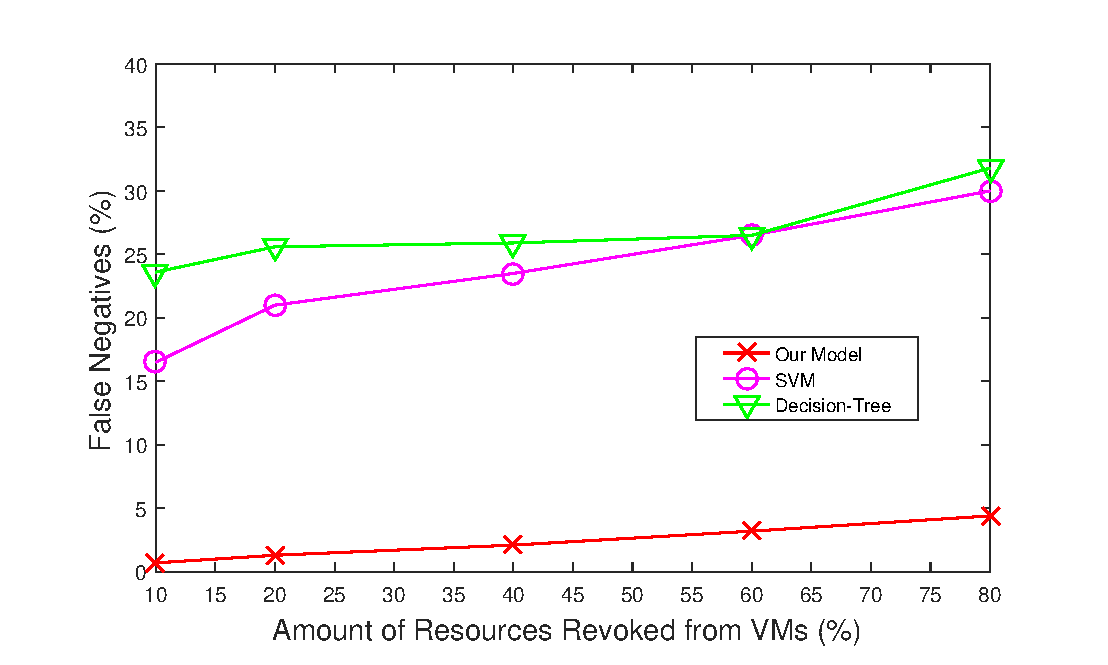
\includegraphics{revfalsenegative.eps}}
    \label{fig1}
    \caption{False negative percentage w.r.t. amount of revoked resources}
\end{figure}


We study in Figures 4, 5, 6, and 7 the performance of our framework with respect to the amount of resources revoked from VMs. The results reveal that our framework is resilient to the decrease in the VMs' resources. More specifically, Figures 4 and 5 show respectively that the average accuracy and attack detection rates obtained by the proposed model at different percentages of revoked resources (from 10\% to 80\%) are 97.02\% and 97.4\%. These results are better than the results obtained using the traditional-SVM (87.14\% for accuracy and 89.54\% for attack detection rate) and Decision-Tree (75.44\% for the accuracy and 79.04\% for attack detection rate). As for the false alarms, Figures 6 and 7 show respectively that the false positive and false negative rates obtained using our model at different percentages of revoked resources (from 10\% to 80\%) are 2.6\% and 2.34\%. These results are also better than the results obtained using  traditional-SVM (10.46 \% for the false positive and 23.5 \% for the false negative) and Decision-Tree (17.28\% for the false positive and 26.68\% for the false negative).

Moreover, Figures. 8, 9, 10, and 11 study the performance of our framework with respect to the amount of resources granted to VMs. These results reveal that our framework is also resilient to the increase in VMs' resources. Figures 8 and 9 show respectively that the average accuracy and attack detection rate obtained by the proposed model at different percentages of granted resources (from 10 \% to 80\%) are 97.36\% and 97.62\%. These results are better than the results obtained using the traditional-SVM (80.66\% for accuracy and 82.36\% for attack detection rate) and Decision-Tree (75.84\% for the accuracy and 77.56\% for attack detection rate). As for the false alarms, Figures 10 and 11 show respectively that the false positive and false negative rates achieved by the proposed model at different percentages of revoked resources (from 10\% to 80\%) are 2.38\% and 2.66\%. These results are also better than the results obtained using the traditional-SVM (17.64 \% for the false positive and 11.68 \% for the false negative) and Decision-Tree (22.44 \% for the false positive and 28.26\% for the false negative).

The reason why our model performs better than the traditional-SVM and Decision-Tree approaches is that the proposed model takes into account the resources adjustments that occur in the VMs' infrastructure. The detection algorithm (Algorithm 2) filters (using the filter obtained from Algorithm 1) the effect of resources adjustments in order to make the collected data (testing dataset) cope with the original infrastructure (on which the training was performed) before passing it to the SVM classifier. This is done by removing the effect of resources adjustments (Algorithm 2, line 5-9). This is unlike the traditional-SVM and Decision-Tree techniques, where the effect of the resources adjustments is totally ignored. Therefore, their accuracy for detecting DoS attacks is affected.

We calculate the percentage of accuracy that can be preserved using our model under changing infrastructure. To do so, we run our model without adjustments applied to the VMs resources. The accuracy of the detection obtained without adjustment was 99.40\%. This result is used as a baseline to calculate the percentage of accuracy that our model can preserve under adjustments. For this purpose, we determine the amount of accuracy preserved under different amounts of adjustments and calculate the average, as in Table 3 for revoking-based adjustments and Table 4 for granting-based adjustments. The results show that the percentage of accuracy that can be preserved is 97.60 \% for the revoking adjustments and 97.96\% for the granting adjustments. This means that, by using our model, the accuracy got decreased under the effect of resources adjustments by only 1.79 \%  for the revoking adjustments and 1.43 \% for the granting adjustments, which has no significant impact and can be neglected.

%[bb=27 14 458 384]

\begin{figure}[!ht]
	\scalebox{0.40}{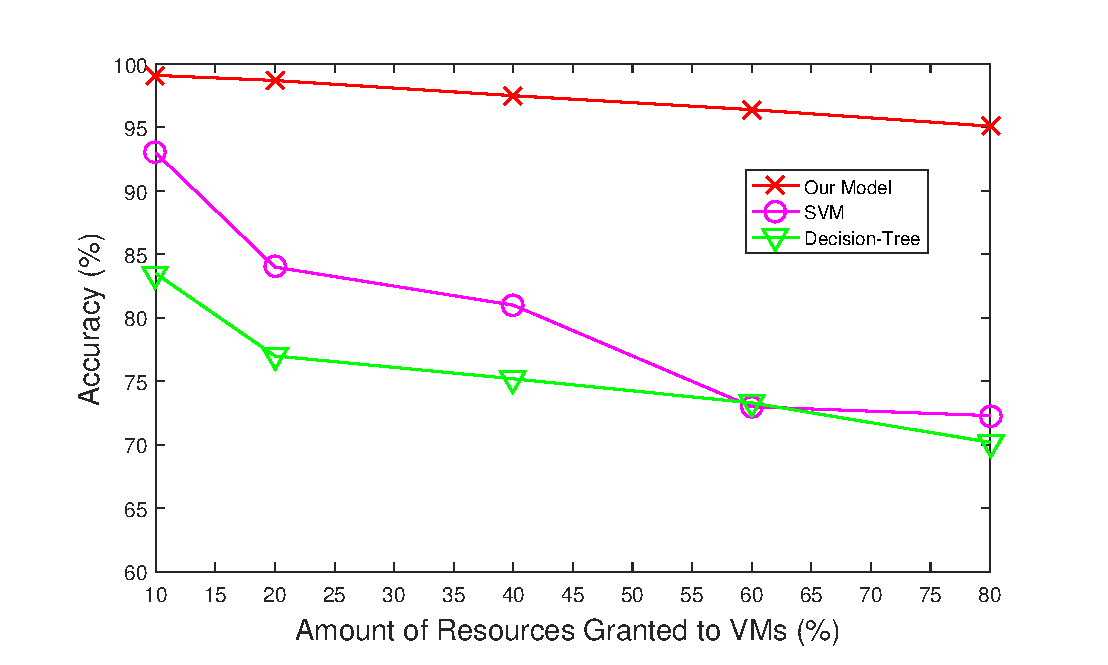
\includegraphics{graaccuracy.eps}}
    \label{fig1}
    \caption{Accuracy w.r.t. amount of granted resources}
\end{figure}

\begin{figure}[!ht]
	\scalebox{0.40}{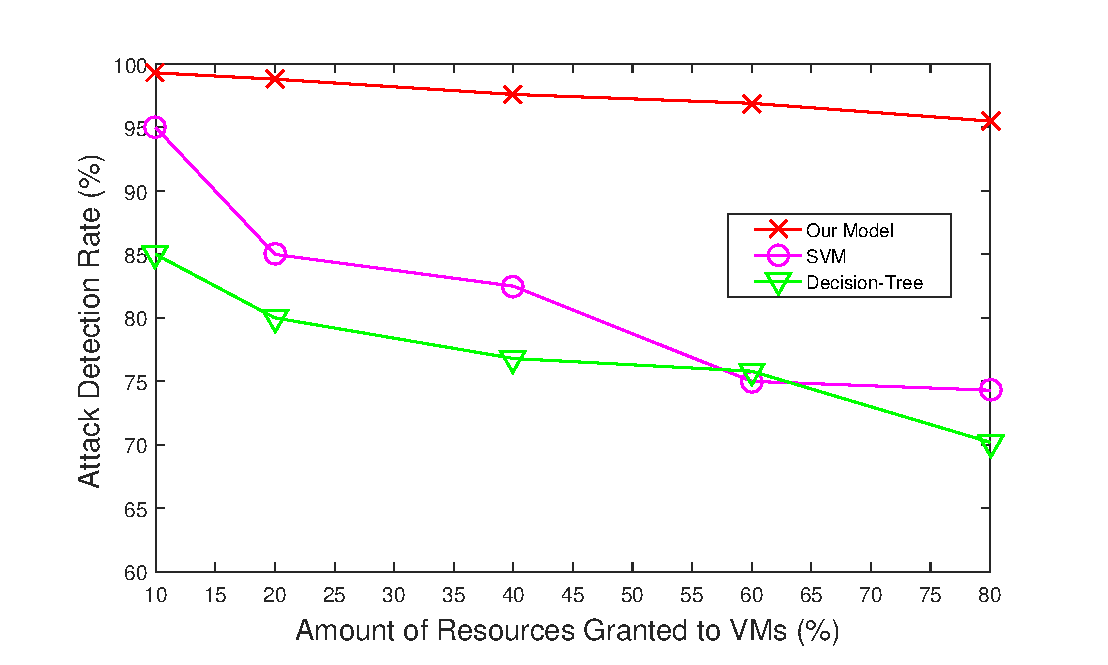
\includegraphics{graattackdetection.eps}}
    \label{fig1}
    \caption{Attack detection rate w.r.t. amount of granted resources}
\end{figure}

\begin{figure}[!ht]
	\scalebox{0.40}{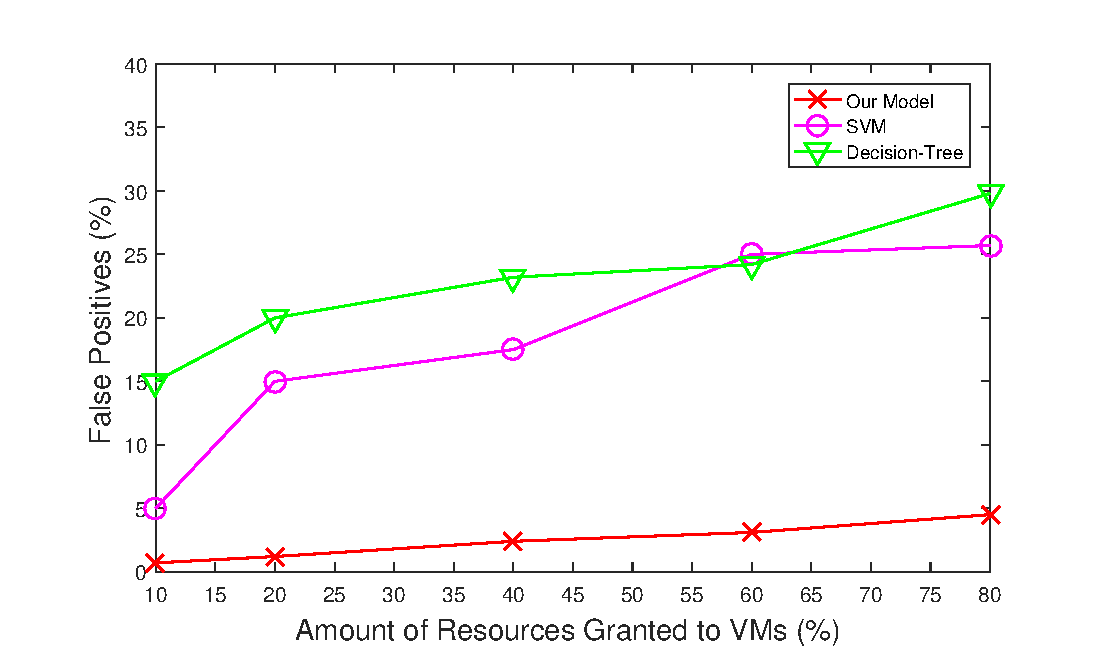
\includegraphics{grafalsepositive.eps}}
    \label{fig1}
    \caption{False positive percentage w.r.t. amount of granted resources}
\end{figure}

\begin{figure}[!ht]
	\scalebox{0.40}{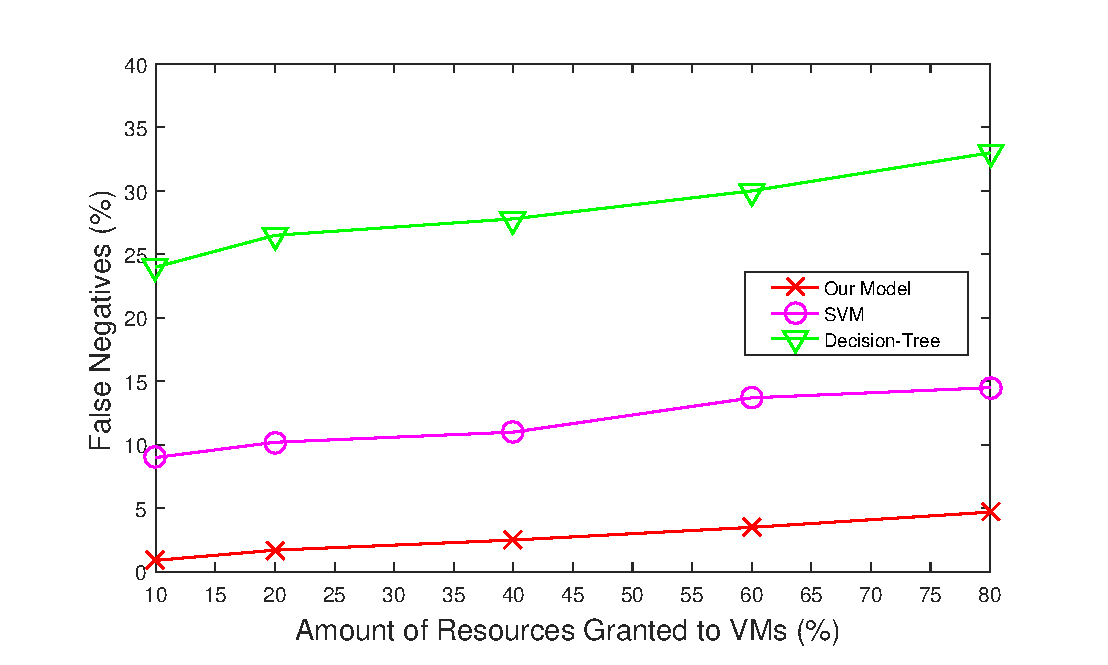
\includegraphics{grafalsenegative.eps}}
    \label{fig1}
    \caption{False negative percentage w.r.t. amount of granted resources}
\end{figure}



\begin{table}[ht]\small
\caption{Amount of accuracy preserved by our model when revoking resources from VMs.}
\centering
 \begin{tabular}{c c}
 \hline
  \textbf{Resources revoked from VMs} & \textbf{Accuracy preserved}\\
  \hline
   10 \%  & 98.79 \% \\
   20 \% &  98.28 \% \\
   40 \% & 98.08 \%  \\
   60 \% & 97.18 \% \\
   80 \% & 95.67 \% \\
    \hline
   \textbf{Average} & 97.60 \% \\
\end{tabular}
\end{table}

\begin{table}[ht]\small
\caption{Amount of accuracy preserved by our model when granting resources to VMs.}
\centering
 \begin{tabular}{c c}
 \hline
  \textbf{Resources granted to VMs} & \textbf{Accuracy preserved }\\
  \hline
   10 \%  & 99.69 \% \\
   20 \% &  99.29 \% \\
   40 \% & 98.08 \%  \\
   60 \% & 96.98 \% \\
   80 \% & 95.77 \% \\
   \hline
   \textbf{Average} & 97.96 \% \\


\end{tabular}
\end{table}
%
%

It should be noticed also that the SVM kernel used in the experiments is the linear kernel. However, our results will not significantly change if we use another non-linear kernel (e.g., Quadratic kernel). In fact, we tested our detection model using different kernels and by considering different values of resources adjustment (granting and revoking adjustments from 10\% to 80\%). Table 5 shows the performance metrics obtained (the average result has been selected) for the different non-linear kernels. It presents the comparisons between different non-linear kernels using the proposed detection model. The results show that there is no significant difference in the false positive, false negative, attack detection and accuracy rates between the different kernel functions.

\begin{table*}[ht]\small \small
\caption{Kernel functions comparison using the proposed detection approach.}
\centering
 \begin{tabular}{c c c c c}
 \hline
 \textbf{Kernel function} & \textbf{Performance metric} & & & \\
    & Accuracy (\%) & Attack detection rate (\%) & False positive rate (\%) & False negative rate (\%)  \\
 \hline
  Linear kernel & 97.19 & 97.51 & 2.49 &  2.50  \\
  Multilayer percepton kernel &97.03 & 97.09 & 2.90 & 2.92  \\
  Quadratic kernel & 97.54 & 97.30 & 2.69 & 2.71  \\
  Polynomial kernel &97.51 & 98.23 &1.99 &2.11   \\
  Gaussian kernel &96.98 &98.05 &1.94 & 2.09  \\
\end{tabular}
\end{table*}

\section{Conclusion}

We present an SVM-based framework for detecting DoS attacks in a virtualized cloud under changing infrastructure. Our solution collects some system metrics to train the SVM classifier to be able to distinguish between normal and malicious (i.e., a DoS attack) activities of the VM. The hypervisor then monitors and quantifies the effect of performing resources adjustments on the collected data. This information is then used to maintain a filter of resources adjustments effect. The filter is used as a preprocessing step prior to classification to get rid of the noise that may show up on the collected data, and that may considerably decrease the accuracy of the detection. Moreover, our solution motivates VMs to declare their current business metrics to the hypervisor, to enable the hypervisor to correlate these metrics with the actual resources' load and decide if it is coherent or not. This increases the possibility of identifying compromised-VMs, trying to claim and consume more resources. Experimental results show that our model performs better than the traditional-SVM and Decision-Tree approaches in the presence of infrastructure adjustments, in terms of false positive, false negative, attack detection and accuracy rate. The results also show that the percentage of accuracy that can be preserved under resources adjustments using our model is 97.60 \% for the revoking adjustments and 97.96 \% for the granting adjustments. Our results also show that the accuracy got decreased under the effect of resources adjustments by only 1.79 \%  for the revoking adjustments and 1.43 \% for the granting adjustments, which has no significant impact and can then be neglected.



%\cite{Arlitt:2016}
%\nocite{oreg,schn,pond,smith,marg,hunn,advi,koha,mouse}

%%%%%%%%%%%%%%%%%%%%%%%%%%%%%%%%%%%%%%%%%%%%%%
%%                                          %%
%% Backmatter begins here                   %%
%%                                          %%
%%%%%%%%%%%%%%%%%%%%%%%%%%%%%%%%%%%%%%%%%%%%%%

\begin{backmatter}

\section*{Competing interests}
  The authors declare that they have no competing interests.

\section*{Authors' contributions}
 AB built the state of the art of the field, defined the objectives of this research,
did the analysis of the current cloud-based detection approaches and their
limitations. He implemented the approach presented in this paper, as well
as the experiments. MB and MD initiated and supervised this research, lead and
approved its scientific contribution, provided general input, reviewed the
article and issued his approval for the final version. All authors read and
approved the final manuscript.

\section*{Authors’ information}

Adel Abusitta is a Ph.D. student in Computer Engineering at Ecole Polytechnique de Montreal, Canada. He holds a M.Sc. degree in computer science from the University of Jordan, Jordan. The main topics of his current research activities are security in Cloud Computing, network security, and authorship analysis.

Martine Bellaiche is Assistant Professor in Department of Computer and Software engineering of Ecole Polytechnique of Montreal.
She received a MSc in Computer Science from University of Montreal in 1985 and the Ph.D in Telecommunications from INRS in 2007. His research
interests are in Network Security with special focus on attack, in Network Sensor Security and cloud computing security.

Michel Dagenais is professor at Ecole Polytechnique de Montreal in the department of Computer and Software Engineering. He authored or co-authored over one hundred scientific publications, as well as numerous free documents and free software packages in the fields of operating systems, distributed systems and multicore systems, in particular in the area of tracing and monitoring Linux systems for performance analysis. Most of his research projects are in collaboration with industry and generate free software tools among the outcomes. The Linux Trace Toolkit next generation, developed under his supervision, is now used throughout the world and is part of several specialized and general purpose Linux distributions.

\section*{Acknowledgements}
 The financial support of the Natural Sciences and Engineering Research Council of Canada is gratefully acknowledged.
%%%%%%%%%%%%%%%%%%%%%%%%%%%%%%%%%%%%%%%%%%%%%%%%%%%%%%%%%%%%%
%%                  The Bibliography                       %%
%%                                                         %%
%%  Bmc_mathpys.bst  will be used to                       %%
%%  create a .BBL file for submission.                     %%
%%  After submission of the .TEX file,                     %%
%%  you will be prompted to submit your .BBL file.         %%
%%                                                         %%
%%                                                         %%
%%  Note that the displayed Bibliography will not          %%
%%  necessarily be rendered by Latex exactly as specified  %%
%%  in the online Instructions for Authors.                %%
%%                                                         %%
%%%%%%%%%%%%%%%%%%%%%%%%%%%%%%%%%%%%%%%%%%%%%%%%%%%%%%%%%%%%%

% if your bibliography is in bibtex format, use those commands:
\bibliographystyle{bmc-mathphys} % Style BST file (bmc-mathphys, vancouver, spbasic).
\bibliography{bibo}      % Bibliography file (usually '*.bib' )
% for author-year bibliography (bmc-mathphys or spbasic)
% a) write to bib file (bmc-mathphys only)
% @settings{label, options="nameyear"}
% b) uncomment next line
%\nocite{label}

% or include bibliography directly:
% \begin{thebibliography}
% \bibitem{b1}
% \end{thebibliography}

%%%%%%%%%%%%%%%%%%%%%%%%%%%%%%%%%%%
%%                               %%
%% Figures                       %%
%%                               %%
%% NB: this is for captions and  %%
%% Titles. All graphics must be  %%
%% submitted separately and NOT  %%
%% included in the Tex document  %%
%%                               %%
%%%%%%%%%%%%%%%%%%%%%%%%%%%%%%%%%%%

%%
%% Do not use \listoffigures as most will included as separate files


%%%%%%%%%%%%%%%%%%%%%%%%%%%%%%%%%%%
%%                               %%
%% Tables                        %%
%%                               %%
%%%%%%%%%%%%%%%%%%%%%%%%%%%%%%%%%%%

%% Use of \listoftables is discouraged.
%%


\end{backmatter}

\end{document}
